\chapter{Semantic Triple Extraction Engine}  \label{ch:5:triple}

\vspace{-2ex}
This section focuses on the Semantic Triple Extraction Engine, particularly on triple representation, implementation, and the key decisions for information extraction.

\section{Motivation}
The aim of this engine was to find a way to extract meaningful information from the article, in particular, information centred around key entities in the article corpus for a certain topic. One of the earlier approaches was to derive a co-occurrence graph of named entities of type 'GPE', 'PER', 'LOC', 'ORG' etc. using Fine-Grained NER (See~\Cref{s:models}) for each topic in a semantic cluster. The limitation of this approach, was that while it was a good indicator of the general entities in a topic, the amount of information extracted from the topic article corpus was not sufficient as no explicit information about \textit{`how'} the entities were related to one another was inferred. In an attempt to extract more `relevant' information indicative to the content discussed in articles of a given topic, the decision was made to extract semantic triples of type \texttt{subject-predicate-object}. The triple serves as a minimal representation for information in an article without losing its context. The process of extracting these relations involved inferring both syntactic and semantic dependencies  between tokens in a sentence, in particular relying on a lexico-semantic approach by making use tokenisation, dependency parsing, part-of-speech tagging and named entity recognition. These triples would then be displayed as a knowledge graph (Refer to \Cref{Knowledge_graph}) for each topic in a semantic cluster.

\section{Key decisions} \label{key_decisions_rel}

In an attempt to capture meaningful nodes (subjects and objects) and relations (predicate), the Semantic Triple Extraction Engine uses phrases instead of words. \Cref{fig:rel_key_decisions} shows the 3 main decisions made for the representation of the triples. 

\begin{figure}[H]
  \centering
  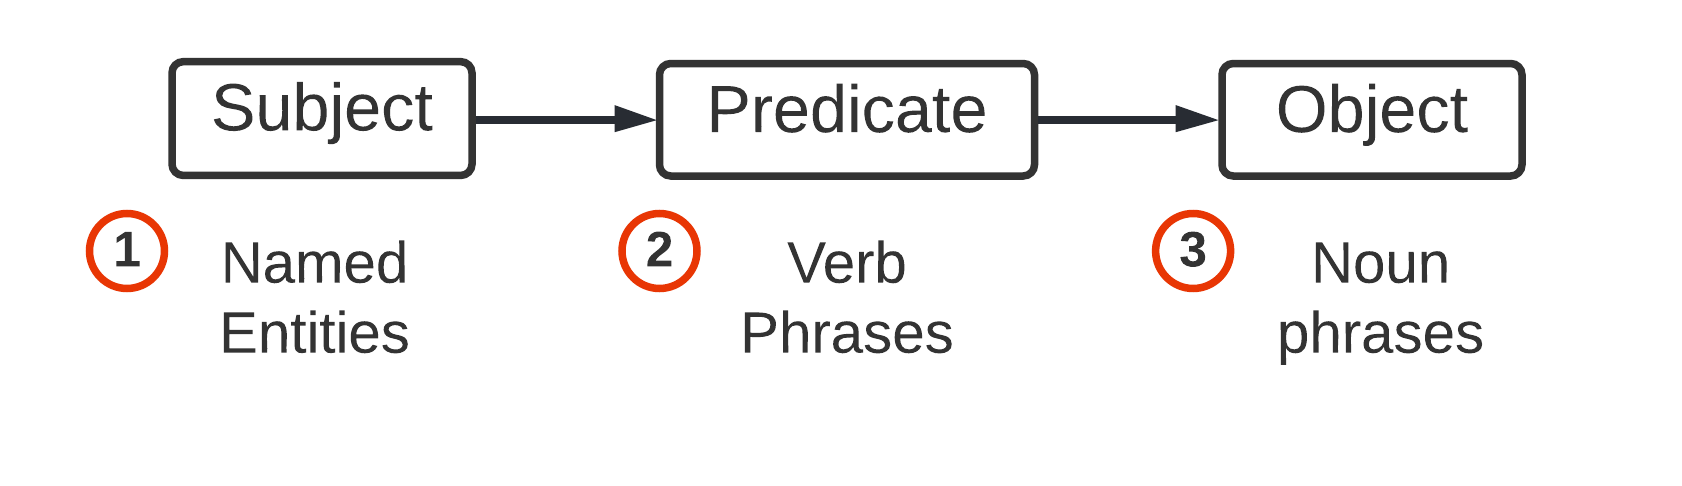
\includegraphics[scale=0.15]{images/relations_kd.png}
  \caption{Decisions for Extracting Semantic Triples}
  \vspace{-1ex}
  \label{fig:rel_key_decisions}
\end{figure}

\begin{enumerate}
  \item \textbf{Named Entities as Subjects:} Given that the end goal is to build a knowledge graph (KG) from these triples, there need to be common `subject' nodes in order to infer information about these entities from the articles and link them to other entities in the graph. For example, if the subject requirement is changed from named entities to simply noun phrases, the engine might extract two triples: one with subject `British Airways' and another with `British Airways spokesperson'. This is not ideal as, although both triples provide information about the named entity `British Airways', they will be displayed as discrete triples. Therefore, using `named entities' as subject grounds the KG to a set of named entities, for which information (semantic triples) can be extracted.
  
  \item \textbf{Verb Phrases as Predicate:} Based on the success of previous studies~\cite{verb_relation_extraction}, the engine relies on the verb-based approach for predicate extraction. It aims to extract a single relation embedded in a sentence that consists of a verb phrase sandwiched between two entities of interest. The motivation for using verb phrases as predicate is that it exploits the structured grammar present in news articles where generally the subject is a person, organisation, place or thing (hence, the use of named entities) and the predicate indicates what the subject is or does, which often involves a `root verb'. These relations of type $subject \rightarrow verb \rightarrow object$ are called SVO triples.
  
  \item \textbf{Noun Phrases as Objects:} Finally, having established SVO semantic triples as the output for this engine, the remaining step is to extract the object phrases. Since the SVO triples follow a pattern of $noun(phrase) \rightarrow verb \rightarrow noun(phrase)$, the object of the triple relies on extracting the noun chunk (using POS tagging) after the verb as the object. 
  
\end{enumerate}

\section{Implementation}

The section highlights the process of extracting the subject, relation, object phrases from the articles in a topic in order to form an entry for the knowledge graph. 

\begin{figure}[H]
  \centering
  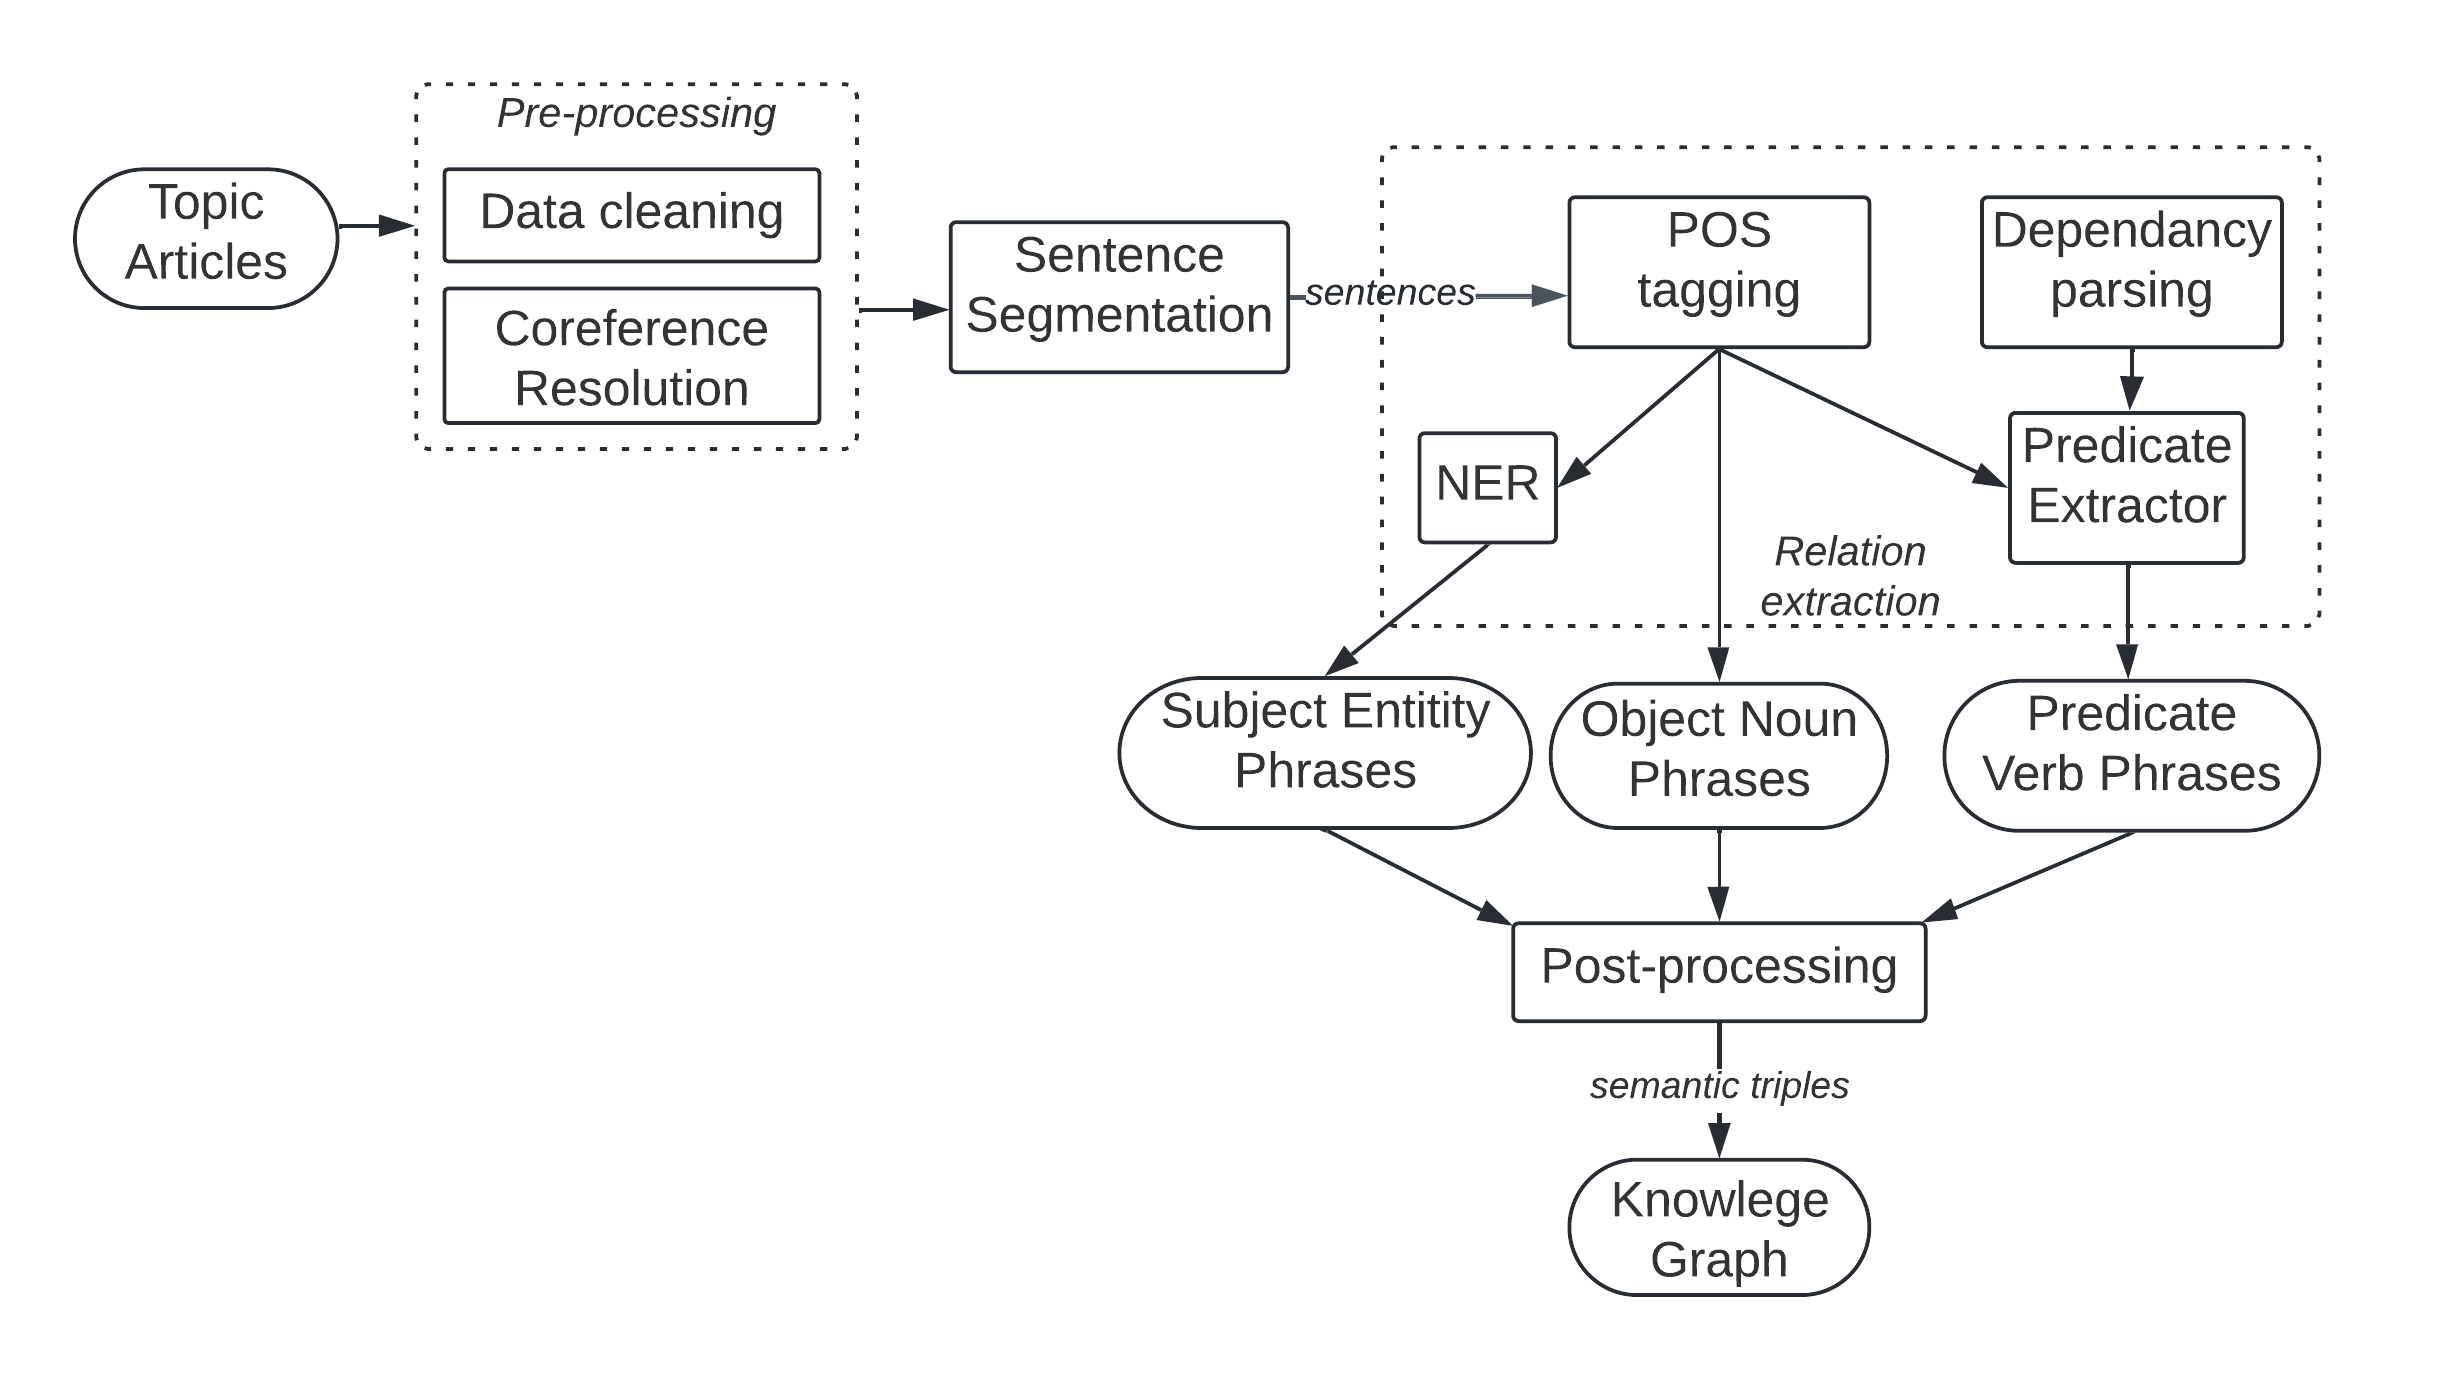
\includegraphics[scale=0.17]{images/ste_imp.png}
  \vspace{-2ex}
  \caption{Overview of Semantic Triple Extraction}
  \label{fig:rel_overview}
\end{figure}

\subsection{Processing Articles}
As seen in~\Cref{fig:rel_overview}, before any information extraction, we need to ensure that the data is correctly preprocessed. For this, the coreference resolved, cleaned articles from~\Crefrange{coref}{data_cleaning} are used. This ensures that all pronouns corresponding to the named entities are resolved, allowing more triples to be extracted from the article corpus with named entities as the `subject'. Extracting triples on a `cleaned' article corpus gets rid of unnecessary text, including stopwords, allowing the model to focus on `semantically rich' words. The \texttt{updated\_stopwords} from~\Cref{data_cleaning} is changed slightly remove any negations such as `not', `won't' etc. While these words were not useful in the Topic Extraction Engine which used a noun-only corpus, negations are relevant when extracting triples as removing these will result in incorrect relations/predicates in the semantic triples and are therefore retained. Each topic article then undergoes sentence segmentation via spaCy's \texttt{SentenceSplitter} to obtain a list of sentences from which the triples can be extracted.

\subsection{Extracting Predicate}

As discussed in \Cref{key_decisions_rel}, the predicate phrases would be extracted as verb phrases. This is done by regex matching of part-of-speech (POS) tags (refer to Appendix \Cref{appendix:pos}) using the following list of matching patterns. 

\begin{minted}[fontsize=\footnotesize, breaklines=True, frame=lines,
  framesep=1mm, baselinestretch=1.0]{python}
verb_patterns = [
  [{'POS':'AUX', 'OP':'?'}, {'POS':'PART', 'OP':'?'}, {'POS':'VERB', 'OP':'+'}, {'POS':'ADP', 'OP':'+'}],
  [{'POS':'VERB', 'OP':'?'}, {'POS':'ADV', 'OP':'*'}, {'POS':'VERB', 'OP':'+'}]
  ]
\end{minted}

% \todonum[inline]{Talk about why these particular regex}
The above list contains two matching patterns using regex operators (See Appendix~\Cref{appendix:ops}) and POS tags to find different permutations of substrings (i.e., verb phrases) to satisfy these patterns. This process does not limit the verb phrase to the `\texttt{VERB}' POS tag, but instead accounts for other relevant information such as auxiliary verbs (`\texttt{AUX}'), adverbs (`\texttt{ADV}') and adposition (`\texttt{ADP}') to be pulled from the sentences as candidate verb phrases in order to retain semantic context. This process is known as `verb chunking'. 

Each of these patterns are based on the commonly occurring grammatical patterns in the English language. For example, the first pattern has an optional requirement (0 or 1 instances) for auxiliary verb (\texttt{`AUX'}) followed by an optional requirement for particle (\texttt{`PART'}) followed by a strict requirement (at least one instance) for `\texttt{VERB}' followed by an optional requirement for `\texttt{ADP}' adposition. Such a pattern allows for the extraction of different combinations of verb chunks such as `has(\texttt{AUX}) been(\texttt{VERB})', `has(\texttt{AUX}) not(\texttt{PART}) been(\texttt{VERB})', `has(\texttt{AUX}) not(\texttt{PART}) been(\texttt{VERB}) in(\texttt{ADP})', `contains(\texttt{VERB})', `belongs(\texttt{VERB}) to(\texttt{ADP})' etc. Similarly, the other pattern tries to extract a verb chunk with an optional `\texttt{VERB}' followed by 0 or more instances of `\texttt{ADV}' (adverbs) followed by at least one instance of `\texttt{VERB}', resulting in verb phrases such as `increasing(\texttt{VERB})', slowly(\texttt{ADV}) increasing(\texttt{VERB})', `is(\texttt{VERB}) slowly(\texttt{ADV}) increasing(\texttt{VERB})' etc. 

These are then filtered to obtain the phrases where the `root' of the sentence is present. This is done using dependency parsing through the spaCy library. Generally, in dependency-based grammars, all words or tokens, in a sentence,  barring one,  are dependent on other words.  This is the root  of the sentence. Most commonly, this word a verb. Therefore, since the scope of relations extracted focuses on the predicate being a verb, the root verb is derived from the dependency tree and all verb phrases containing the root verb are retained. Given the regex pattern matching criteria discussed above, each sentence might result in multiple root verb phrases, for example, one with just the root verb (e.g 'calling'), one with the auxiliary verb (e.g. 'are'), root verb (e.g. 'calling') and adposition (e.g. 'for') as shown in~\Cref{verb_phrases}. In order to extract the most informative coherent relations, the longest verb phrase is selected. 

\begin{figure}[H]
\centering
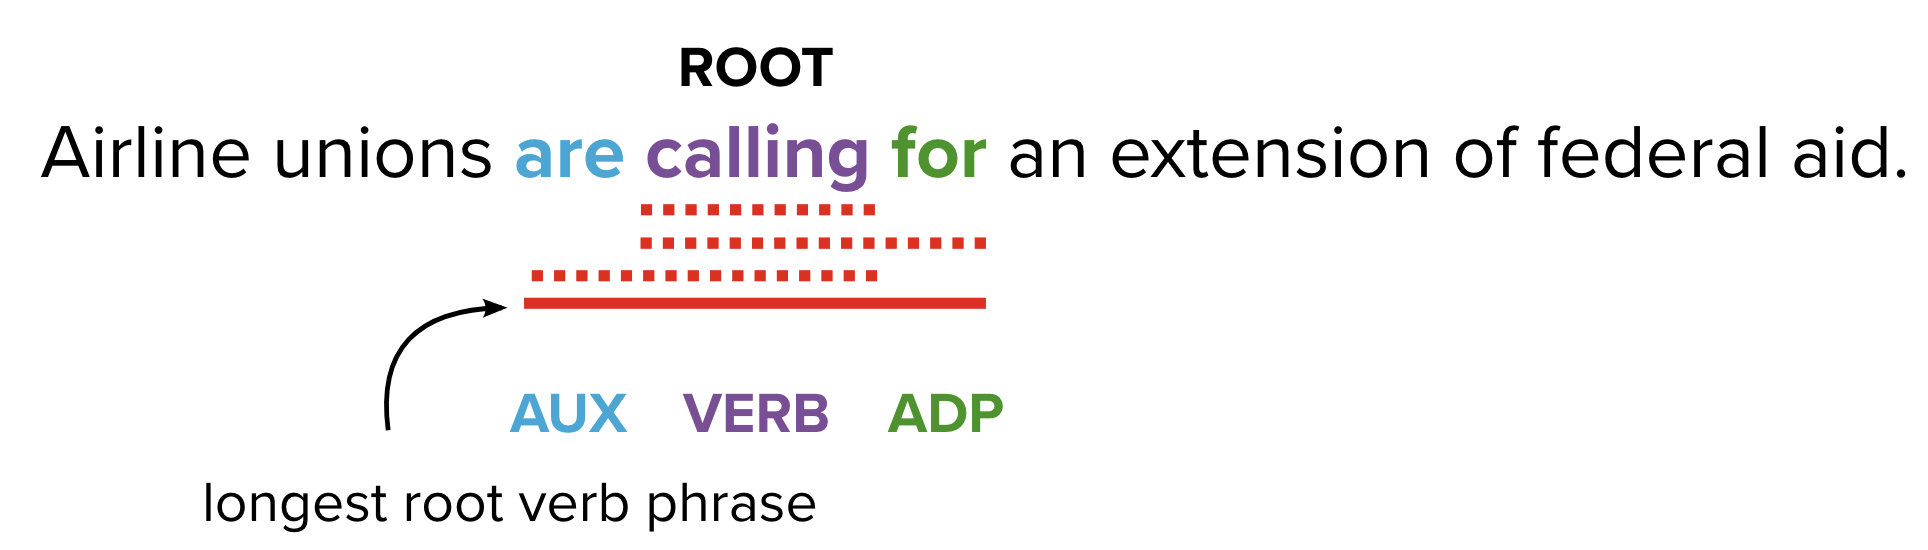
\includegraphics[scale=0.3]{images/verb_phrases.png}
\caption{Verb phrases extracted from an example sentence from article corpora}
\label{verb_phrases}
\end{figure}

\subsection{Extracting Subject and Object} \label{extracting_subj_obj}
As discussed in \Cref{key_decisions_rel}, the `subject' and `object' are noun phrases (NP), particularly entity phrases for `subject'. Therefore, in order to derive these, the `noun chunks' are extracted from the sentence using POS tagging and chunking from the spaCy pipeline. These `noun chunks' are base noun phrases with no nested NP and relative clauses~\cite{spacy} and are returned as a list of \texttt{Spans}~\cite{spacy}, which are essentially slices of the sentence and contain information such as the `start' and `end' position of the sentence `chunk' (phrase). \Cref{alg:subject_relation} outlines the process of extracting the subject and object phrases in the semantic triple.

\begin{algorithm}[H]
  \caption{Outline of Triple Extraction Procedure}
  \label{alg:subject_relation}
  \begin{algorithmic}   
  \Function{GetSubjectAndAugmentedPredicate}{$verbPredicate, validEnts, nounPhrases$}
    \ForAll {$np \in nounPhrases$}
    
      \If {$np.start < verbPredicate.start$}
      \State $ents \gets np.containsAny(validEnts)$ 
      \Comment{all entities in np}
        \If {$ents.length == 0$}
        \State $continue$
        \EndIf
      \State $subjectEnt \gets ents.sort(key = lambda \ e: e.start)[0]$
      \State $remnantNp \gets np.partition(subjectEnt).last$ 
      \Comment remnant phrase right of subject
      \State $augmentedPred = remnantNp + verbPredicate $
      \State $break$
      \EndIf
    \EndFor
    \State \Return $subjectEnt, augmentedPred$
  \EndFunction

  \Function{GetObject}{$verbPredicate, nounPhrases$}
    \ForAll {$np \in nounPhrases$}
      \If {$np.start > verbPredicate.start$}
      \State $object \gets np$ 
      \State $break$
      \EndIf
    \EndFor
    \State \Return $object$
  \EndFunction
\end{algorithmic}
\end{algorithm}

\vspace{-3ex}
\subsubsection{Subject Entity and Augmented Predicate}
In order to extract the subject phrase, we get the first noun phrase (NP) that occurs before (to the left of) the verb phrase (i.e., predicate) as well as contains at least one of the selected set of named entities (i.e., \texttt{valid\_entities}). The named entities contained in the noun phrase (\texttt{np}) are stored as candidates for the subject (\texttt{ents}). The \texttt{valid\_entities} are derived by performing Named Entity Recognition (NER) on the sentence using the Fine-Grained NER model as detailed in~\Cref{alg:named_ents}. As mentioned previously in~\Cref{s:models}, the model returns 16 semantic types (See~\Cref{appendix:semantic_types}). Some of these entity types can result in unnecessary and irrelevant triples with, for instance, (`two', \texttt{`CARDINAL'}) as the subject node. Therefore, in a slight adjustment to the named entity extraction procedure detailed in~\Cref{alg:named_ents}, a set \texttt{ignore\_entity\_types}, containing \texttt{`DATE', `TIME', `CARDINAL', `PERCENT'} and \texttt{`QUANTITY'}, is passed to omit extracted entities of these types. This does not mean that information about these entities is completely ignored as they are likely to be extracted as object phrases when in reference to a `valid' subject named entity. 

Of the subject candidates, the first occurring (based on position of the entity \texttt{Span}) is selected as the subject phrase. As mentioned in~\Cref{key_decisions_rel}, the aim is to have just the named entity as the subject to facilitate connectivity of triples in the knowledge graph (KG). However, we do not want to lose the other semantic information in the subject phrase. Therefore, the subject phrase is split into the entity and the remnant phrase \textit{after} the entity, which is then prepended to the predicate. This way the information conveyed by the noun phrase is conserved, but the subject node is maintained as an entity. For example, for the triples: \texttt{(`Transat investors', `choose receiving', `cash payment')} and \texttt{(`Transat', `to become part of', `Air Canada')}, splitting the $1^{st}$ triple's subject to get `Transat' and `investors' and augmenting the predicate with the latter to get the updated triple: (`Transat', `investors choose receiving', `cash payment') results in a common subject node between the triples as shown in~\Cref{fig:transat_after}. Without this, the KG would be poorly connected with 2 distinct triples as shown in~\Cref{fig:transat_before}.
  
\begin{figure}[H]
  \begin{minipage}{0.5\linewidth}
  \centering
  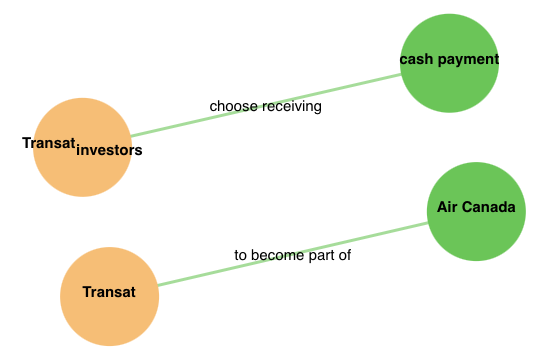
\includegraphics[width=0.8\linewidth]{images/kg_transat.png}
  \caption{KG snippet before predicate augmentation}
  \label{fig:transat_before}
  \end{minipage}
  \hfill
  \begin{minipage}{0.5\linewidth}
  \centering
  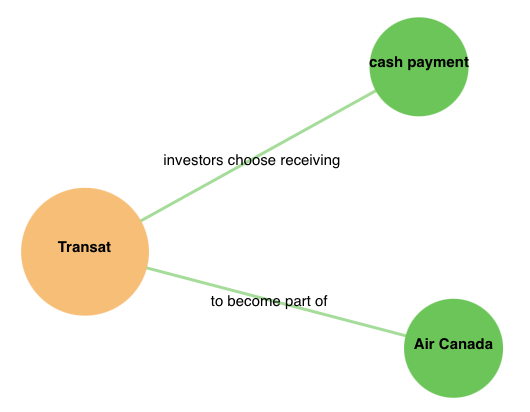
\includegraphics[width=0.8\linewidth]{images/kg_transat_correct.png}
  \caption{KG snippet after predicate augmentation}
  \label{fig:transat_after}
  \end{minipage}
\end{figure}

\vspace{-4ex}
\subsubsection{Get object phrase}
Getting the object is fairly simple as shown in \Cref{alg:subject_relation} and involves getting the first (closest in position) `noun phrase' after the `predicate' (the longest root verb phrase).

\subsubsection{Post-processing}
Once the semantic triples are obtained from the article corpus for each topic, they undergo filtering. This involves ensuring that all components of the triple are not null (or empty string) and the triples where the relation/predicate contain words like ``said" and ``told" (including all their grammatical forms) are omitted. This is done because, very commonly in news articles, direct quotes are made by entities of the forms ``$\langle quote \rangle, \ said \ \langle entity \rangle$" or ``$ \langle entity \rangle, said \big \langle quote \rangle$". The root verb extracted by the engine in these cases would be `said' and the triples would be of type ($\langle junk \rangle, \ said, \ \langle entity \rangle$) or ($\langle entity \rangle, \ said, \ \langle junk \rangle$) respectively, where $\langle junk \rangle$ implies incoherent subject or object nodes, resulting in poor relations that do not add to the quality of the relations extracted for a particular entity. 

Furthermore, in order to ensure conciseness of the triples and eliminate redundancy, any common substring (likely to occur from noun phrase chunking and verb phrase regex matching) is eliminated by calculating the longest common substring containing complete words between the subject and object as well as (augmented) predicate and object and removing it from the object phrase. 


\section{Results and Discussion}

% \todonum[inline]{Show types of relations extracted with dep parsing and otherwise}
% \todonum[inline]{Talk about the object-relation-subject gotcha.}

The advantage of using the approach discussed in~\Cref{extracting_subj_obj} to extract the semantic triples is that it avoids the stringent dependency of the `subject' and `object' phrases on their actual dependency tags (in the dependency grammar) (See \Cref{dependency_grammar}), instead using dependency parsing only to extract the root verb in the sentence, and getting the subject and object based on the position of `noun chunks' before and after the root verb. An alternate approach was tried relying on the dependency grammar structure to find the subject and object which did not always yield great results as the information extracted was heavily influenced by the grammatical structure of the sentence, which, in the case of news articles, can get very complex due to several nested dependencies. For the knowledge graph, ultimately, the relations extracted need to focus around different named entities. This means that more often than not, relevant information about entities was lost \hl{due to the `named entity' being identified as the object dependency (`obj') in the grammar with a dependency tag such as \texttt{`iobj', `dobj'} instead of having one of the subject tags (`subj') such as \texttt{`nsubj', `csubj', `nsubjpass',	`csubjpass'}}(See Appendix \Cref{appendix:deps}). \hl{The dependency sentence structure is commonly of type `subj'-`verb'-`obj' or `obj'-`verb'-`subj, where `subj' and `obj' include all the variants of the subject and object dependency tags respectively. Our current approach accommodates both these grammatical structures as it only enforces that the `subject' in the semantic triple is a named entity and therefore, can have either `subj'  or `obj' (including variants) as the dependency tag. }



\subsubsection*{Knowledge graph of Semantic Triples}

After extracting the qualifying semantic triples for each topic (in cluster), a force-directed (knowledge) graph of these triples is generated by the visualisation tool. \Cref{fig:triples_travel2021} shows the graph for Cluster 1 in Travel 2021 (See \Cref{fig:topics_travel2021}) which has a single topic `tourism, reopening, government'. 

\vspace{-1ex}

\begin{figure}[H]
  \centering
  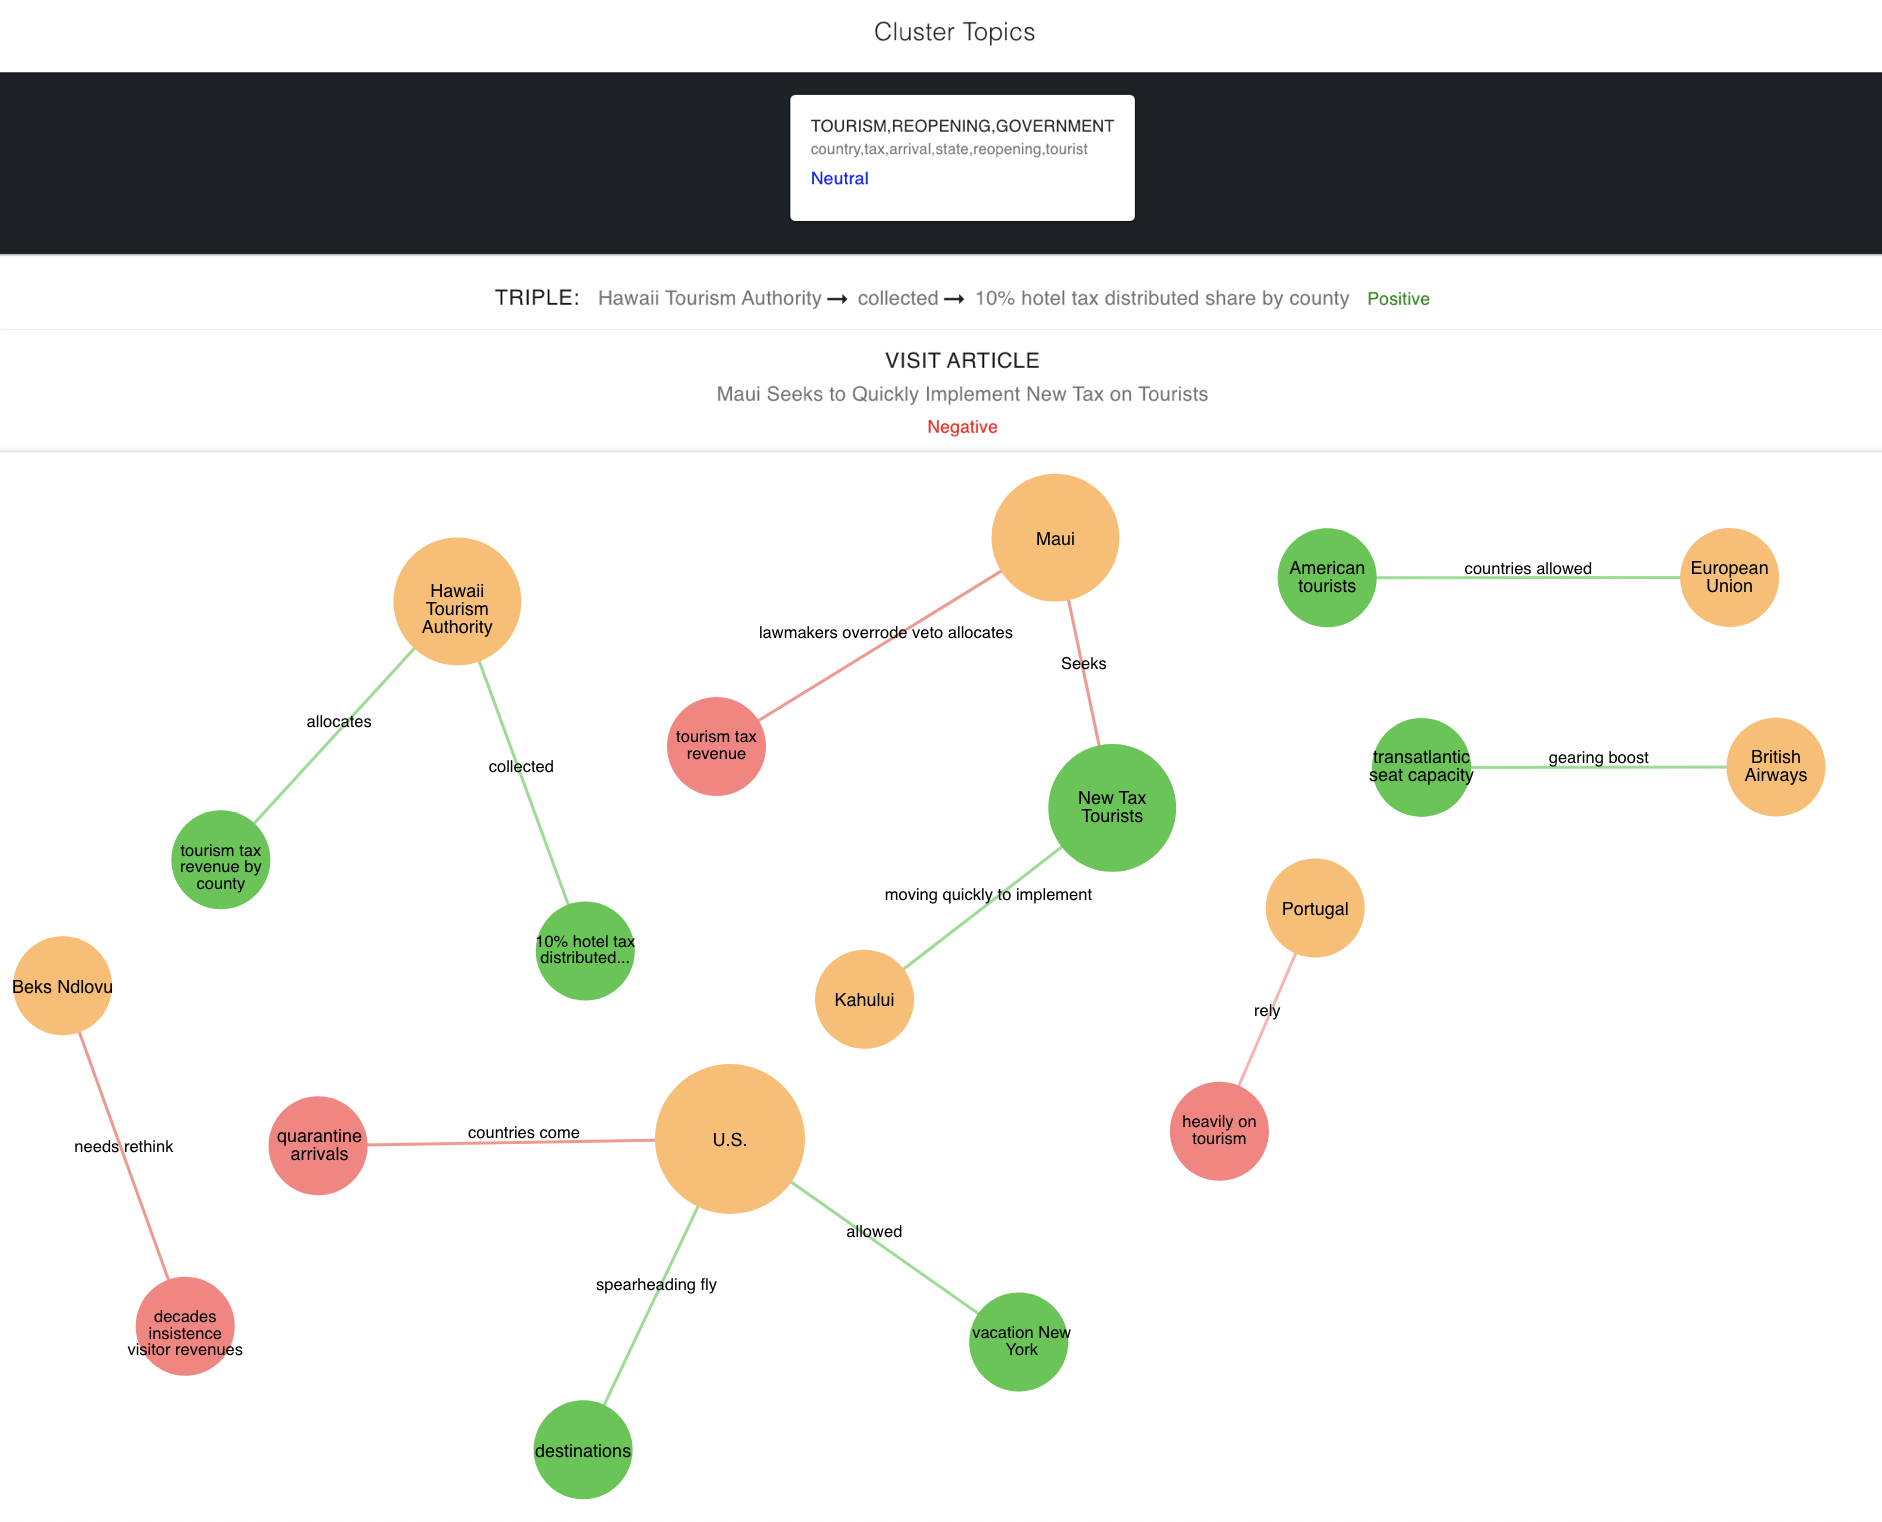
\includegraphics[width=\linewidth]{images/travel2021_triples_witha.png}
  \caption{Knowledge Graph for topic `tourism, reopening, government' in Cluster 1 in `Travel 2021'}
  \vspace{-1ex}
  \label{fig:triples_travel2021}
\end{figure}



\Cref{fig:triples_travel2021} shows the graph generated by the visualisation tool for Cluster 1 (C1) which has a single topic `tourism, reopening, government'. The `subject' nodes (i.e., named entities) are in orange, the `object' nodes are in green (indicating `positive' sentiment) or red (indicating `negative' sentiment) and the edges joining these represent the `predicate'. Clicking on the predicate shows the entire semantic triple (and the corresponding `triple sentiment') as well as the article (and the article `sentiment') from which the triple was extracted. The size of a node is determined by the degree of edges incident upon it, thereby making it easier to identify the key entities in a topic. For example, we see that the `Hawaii Tourism Authority', `U.S.' and `Maui' have more triples associated with them as opposed to `Portugal', making the former nodes bigger and therefore stand out more from a visual aspect. Additionally, we can see the interconnectivity of the nodes with the example of `Maui' and `Kahului' which both share the `object' node `New Tax Tourists'. These gives us the insight that both `Maui' and `Kahului' which are islands in Hawaii have implemented a new tourist tax, which is further verified at by the triple: `Hawaii Tourism Authority' $\rightarrow$ `allocates'  $\rightarrow$ `tourism tax revenue by county'.

As mentioned prior, the colour of nodes is a representation of the sentiment of the triple. This may not always coincide with the sentiment of the article. The motivation for this was to see the general sentiment surrounding an entity which can come from the entity being mentioned in different contexts in multiple articles. For instance, the `European Union has a `positive' sentiment associated with it as the information we have on it is that EU countries allowed `American tourists'. An important thing to note is that the sentiment is quite context dependent, for example, going back to the triples `Maui' $\rightarrow$ `seeks'  $\rightarrow$ `new tax tourists' and `Kahului' $\rightarrow$ `moving quickly to implement' $\rightarrow$ `new tax tourists', we see that the former has a `negative' sentiment (implied by the red `predicate' line joining the nodes)  while the latter has a `positive' sentiment associated to it. This is because `seeking tax' presents negative connotations whilst `moving quickly to implement' has connotations of efficiency and enthusiasm which are positive.


\subsection*{Limitations}

One of the main limitations Semantic Triple Extraction Engine is that, given its verb-based approach, it extracts a single relation embedded in a sentence composed of a (root) verb phrase sandwiched between two entities of interest. 
News articles lend themselves to a sentence structure that is relatively complex with several subjects and objects in a single sentence. Often, trying the maximise information extraction from a single sentence can lead to redundancies and incoherent semantic triples. Therefore, the focus of this model is that it aims to extract a single relation in a sentence provided the sentence mentions a named entity. 

Another limitation of the engine comes from the performance of the spaCy library used for sentence segmentation, POS tagging, dependency parsing as well as the state-of-the-art AllenNLP models: SpanBERT for coreference resolution, Fine-grained Named Entity Recognition and RoBERTa Stanford Sentiment Treebank (See~\Cref{s:models}) used for resolving coreferences in the article corpus in preprocessing, extracting the named entities from the sentences for the `subject' node and performing sentiment analysis on the articles, topics and triples respectively. The performance of these models have a huge effect in the performance of the Relation Extraction Engine. 

